\lecture{9. Written on Their Hearts}{09}

%------------------------------------------------------------------------------
\section{Introduction}

%--------------------------------------
\begin{frame}{Wilhelm Wundt}
\framesubtitle{The father of modern psychology}
\begin{center}
	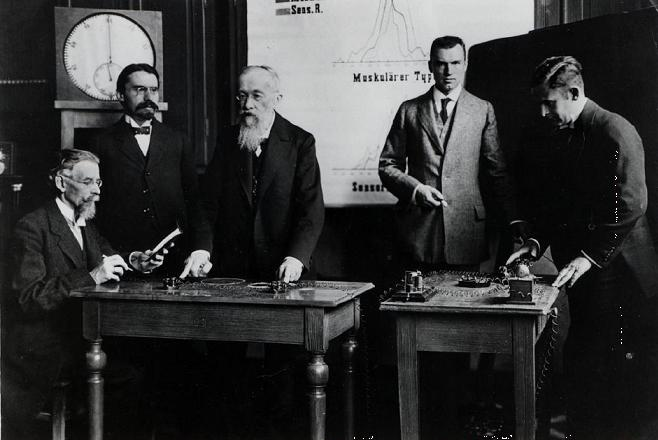
\includegraphics[width=0.8\textwidth]{figures/wundt.jpg}
\end{center}

\note{09:30}
\note[item]{Wilhelm Wundt, Institute for Experimental Psychology, University of Leipzig in Germany in 1879.}
\note[item]{Separated psychology from philosophy by emphasizing experimentation.}
\note[item]{Wundt argued that conscious mental states could be scientifically studied using introspection.}
\note[item]{He trained psychology students to make observations.}
\note[item]{Introspection was an unreliable method of investigation.}
\note[item]{Introspection could not be used to study children or animals.}
\note[item]{Complex topics, such as learning, development, mental disorders, and personality, could not be investigated.}
\note[item]{Yet, to this day, introspection is seen as the key to self-discovery}
\note[item]{God knows more about our psyche than we do.}
\end{frame}

%--------------------------------------
\begin{frame}{God wants a relationship with people}
\framesubtitle{Jeremiah 31:31-34}
	\keyversehiglight{I will put my law within them, and I will write it on their hearts}
	
\note{09:32}
\end{frame}

%--------------------------------------
\begin{goals}
\goal Know what your `heart' is and how the New Covenant is `written' upon
it
\goal Determine some internal and external ways to evaluate our hearts
\goal Commit to continual heart transformation as a way to draw closer to
God

\note{09:34}
\end{goals}

%------------------------------------------------------------------------------
\section{What is the heart?}

%--------------------------------------
\begin{frame}{What is the heart?}
\framesubtitle{}
The heart is an organ
\begin{quote}
`The heart is a muscular organ in humans and other animals, which pumps blood through the blood vessels of the circulatory system.  Blood provides the body with oxygen and nutrients, and also assists in the removal of metabolic wastes.' 
\end{quote}

The heart is a symbol
\begin{quote}
`[The heart] denotes a person's center for both physical and emotional-intellectual-moral activities; sometimes it is used figuratively for any inaccessible thing.'
\end{quote}

\note{09:36}
\note[item]{Ancients didn't view the association between the heart and thoughts, emotions as a symbol.}
\end{frame}

%--------------------------------------
\begin{frame}{The New Covenant vs. the Old}
\framesubtitle{Jer. 31:31-34}

\begin{description}[from the least to the greatest]
\item[I will put my law within them] genuine obedience
\item[I will write it on their hearts] inward commitment
\item[I will be their God] a new focus
\item[they shall be my people] it's no longer physical Israel
\item[\ldots they shall all know me] faith not genealogy
\item[from the least to the greatest] there's no distinctions
\item[I will forgive their iniquities] more than overlooking sins
\end{description}

\note{09:40}
\note[item]{write it on hearts -- not tablets.  Israelites should have done this (law `when you rise up and lay down').  Christians will get it right.}
\note[item]{God's covenant will become part of who we are}
\note[item]{Again, a separation existed in the Old Covenant.}
\note[item]{The separation was partly institutional, but mostly it was that people didn't internalize God's law.}
\end{frame}

%--------------------------------------
\begin{frame}{Our heart can be strong}
\framesubtitle{2 Corinthians 4:16-18}

\begin{itemize}
	\item We can (and will) get old, physically.
	\item But, our heart can rise above our physical limitations.
\end{itemize}

\note{09:44}
\note[item]{This also implies that our heart is something more than our mental faculties, which can also dissipate with age.}
\end{frame}

%------------------------------------------------------------------------------
\section{How to evaluate our hearts}

%--------------------------------------
\begin{frame}{God judges us by our heart}
\framesubtitle{1 Samuel 16:7}

\begin{itemize}
	\item Man looks on the outward appearance
	\item The Lord looks on the heart
	
\end{itemize}

\note{09:48}
\note[item]{How you look has very little to do with who you are.}
\note[item]{When people say, ``God knows my heart'', they are misusing this principle.}
\note[item]{What they mean is, ``I may be behaving in a manner inconsistent with the Bible, but inside I'm very sincere.''}
\note[item]{It's not possible to separate your heart from your actions.}
\note[item]{Your actions certainly speak more about your heart than your physical appearance.}
\note[item]{For example, Saul}
\end{frame}

%--------------------------------------
\begin{frame}{Law outside your heart is useless}
\framesubtitle{Hebrews 4:1-10}

\begin{itemize}
	\item The Law didn't benefit the Israelites because they didn't believe it.
	\item And it kept them out of the promised land.
\end{itemize}

\note{09:52}
\note[item]{Belief plays such a central role.}
\note[item]{It's a shame that the Calvinists have made it a `bad' word among NT Christians.}
\note[item]{Don't let their false teachings dissuade you from emphasizing the importance of belief.}
\end{frame}


%--------------------------------------
\begin{frame}{Knowing if your heart is good}
\framesubtitle{1 John 3:19-24}

\begin{itemize}
	\item God's love and forgiveness is greater than our lingering guilt of sin. 
	\item When we believe in Jesus, love one another, keep His commandments, and have a relationship with the Spirit\ldots
	\item Then, our hearts will feel clean and we'll have confidence in our relationship with God.
	\item You can't have a good heart without love. (Deut. 10:12-22)
\end{itemize}

\note{09:56}
\note[item]{Your conscience, if it's sensitive, could always be niggling you that there is some imperfection in you.}
\note[item]{But, you need to have confidence that God has cleansed you.}
\note[item]{You can bolster that confidence by following the principles outlined in vs.23-24.}
\note[item]{Remember, we're striving for faithfulness not perfection.}
\note[item]{Deut. 10:12-22 Talks about how when you set your heart to God's law, then you love god and your neighbor}
\end{frame}

%------------------------------------------------------------------------------
\section{Transforming our hearts}

%--------------------------------------
\begin{frame}{You can choose your heart}
\framesubtitle{Ezra 7:10}

Ezra \emph{set} his heart to
\begin{itemize}
	\item study
	\item teach
	\item do
\end{itemize}

\note{10:00}
\note[item]{You read about David, and you think, ``I wish I was a man after God's own heart.''}
\note[item]{The simple answer is, ``You can be!''}
\note[item]{Ezra decided to have a righteous, spiritual life, and God helped him get there.}
\note[item]{You can do the same.}
\end{frame}

%--------------------------------------
\begin{frame}{Decide to be Different}
\framesubtitle{Romans 12:1-2}

\begin{itemize}
	\item{The world would not choose to be a living sacrifice, because it doesn't see the benefits.}
	\item{The Christian is transformed by first rejecting worldliness in his mind.}
	\item{That transformation brings about discernment.}
\end{itemize}

\note{10:04}
\note[item]{You're not going to make the right choices unless you're humble enough to reject your way of doing things in favor of God's way of doing things.}
\end{frame}

%--------------------------------------
\begin{frame}{Law inside your heart is revealing}
\framesubtitle{Hebrews 4:11-13}

\begin{itemize}
	\item Divides the soul and spirit
	\item Discerns the thoughts and intentions of your heart.
\end{itemize}

\note{10:08}
\note[item]{People spend a lot of time trying to figure themselves out.}
\note[item]{Self-help books are everywhere.}
\note[item]{But, introspection, by itself, can only take you so far.}
\note[item]{Introspection guided by God's word, however, will take you to heaven.}
\note[item]{You can't overemphasize the importance of meditating on God's word.}
\note[item]{That's one of the reasons why, when we preach or teach a class, we should prepare our scriptures well in advance.}
\note[item]{You have to have time to think about the passages.}
\note[item]{A genuine understanding doesn't just happen immediately.}
\end{frame}

%------------------------------------------------------------------------------
\section{Review}

\begin{frame}{Written on Their Hearts}
	\begin{center}
		God wants a relationship with people from their hearts.
	\end{center}
	The heart
	\begin{itemize}
		\item Your heart \emph{is} you.
		\item Your heart was built to be the home for God's law.
		\item Your heart grows as you grow close to God.
	\end{itemize}
	Evaluate your heart
	\begin{itemize}
	\item God judges us by our heart.
	\item Belief is a test of the heart.  Israel failed that test.
	\item Other tests: ``love one another'', ``keep my commandments''
	\end{itemize}
	Transform your heart
	\begin{itemize}
	\item You can choose your heart.
	\item Reject worldliness in favor of being a living sacrifice.
	\item Meditate on God's word to refine your heart.
	\end{itemize}
	
\note{10:12}
\end{frame}

%--------------------------------------
%\begin{frame}{Frame 1}
%\framesubtitle{Passage 1}
%
%\begin{columns}[c]
%\begin{column}{0.6\textwidth}
	%
\includegraphics[draft, width=\columnwidth]{figures/dummy.png}
%\end{column}
%\begin{column}{0.4\textwidth}
	%Point 1\ldots
	%\begin{itemize}
		%\item Subpoint 1
	%\end{itemize}
%\end{column}
%\end{columns}
%
%\note{09:38}
%\note[item]{King James says bowels}
%\end{frame}
%
